Skuteczne wdrożenie nowego systemu zarządzania danymi wymaga dobrze przemyślanego planu działań. Kluczowe jest określenie założeń projektowych, podziału ról w zespole oraz harmonogramu prac, które zapewnią sprawną realizację kolejnych etapów. W tym rozdziale przedstawione zostały metody organizacji pracy w celu efektywnego zarządzania projektem i osiągnięciem założonych celów w optymalnym czasie.

\section{Podstawowe założenia}

Każde rozwiązanie technologiczne powinno być nie tylko odpowiedzią na konkretne wyzwanie, ale także uwzględniać realia organizacyjne, w których ma funkcjonować. W przypadku \gls{cinn} kluczowym wyzwaniem było usprawnienie zarządzania danymi związanymi z organizacją wydarzeń – przy jednoczesnym zachowaniu zgodności z istniejącą infrastrukturą technologiczną i minimalizacji dodatkowych kosztów inwestycyjnych.

\gls{pw} korzysta z ekosystemu Microsoft 365, co oznacza, że wszelkie nowe rozwiązania musiały być bezproblemowo z nim zintegrowane. Zastosowanie narzędzi takich jak \gls{powerautomate}, \gls{powerquery} i \gls{forms} pozwala na automatyzację procesów bez konieczności wdrażania zewnętrznych systemów. Ostatecznym celem było nie tylko zmniejszenie obciążenia pracowników poprzez eliminację ręcznego przetwarzania danych, ale także zapewnienie długoterminowej łatwości utrzymania systemu – aby jego obsługa i rozwój nie wymagały specjalistycznej wiedzy technicznej.

Dodatkowo, system musiał zachować intuicyjny proces rejestracji dla uczestników wydarzeń oraz umożliwiać pracownikom łatwy dostęp do uporządkowanych danych. W ten sposób rozwiązanie miało nie tylko usprawnić operacje wewnętrzne, ale także zwiększyć przejrzystość i wygodę użytkowników końcowych.


\section{Zespół Projektowy} 
Projekt wdrożenia systemu automatyzacji zarządzania danymi wydarzeń w \gls{cinn} był realizowany przez dwuosobowy zespół. Odpowiedzialność za analizę, projektowanie, implementację oraz testowanie rozwiązania spoczywała na autorce niniejszej pracy, która pełniła rolę głównego projektanta oraz wykonawcy.

Funkcję kierownika formalnego pełniła Agnieszka Lewandowska, której rola koncentrowała się na nadzorowaniu przebiegu projektu oraz koordynacji działań związanych z jego wdrożeniem w strukturze organizacyjnej \gls{inin}. Praca obejmowała regularne konsultacje oraz testy funkcjonalności, co umożliwiło dostosowywanie systemu do potrzeb użytkowników końcowych.

\section{Plan Pracy}
Realizacja projektu została podzielona na kilka kluczowych faz, każda z jasno określonymi kamieniami milowymi. 

\begin{figure}[!hb]
	\centering 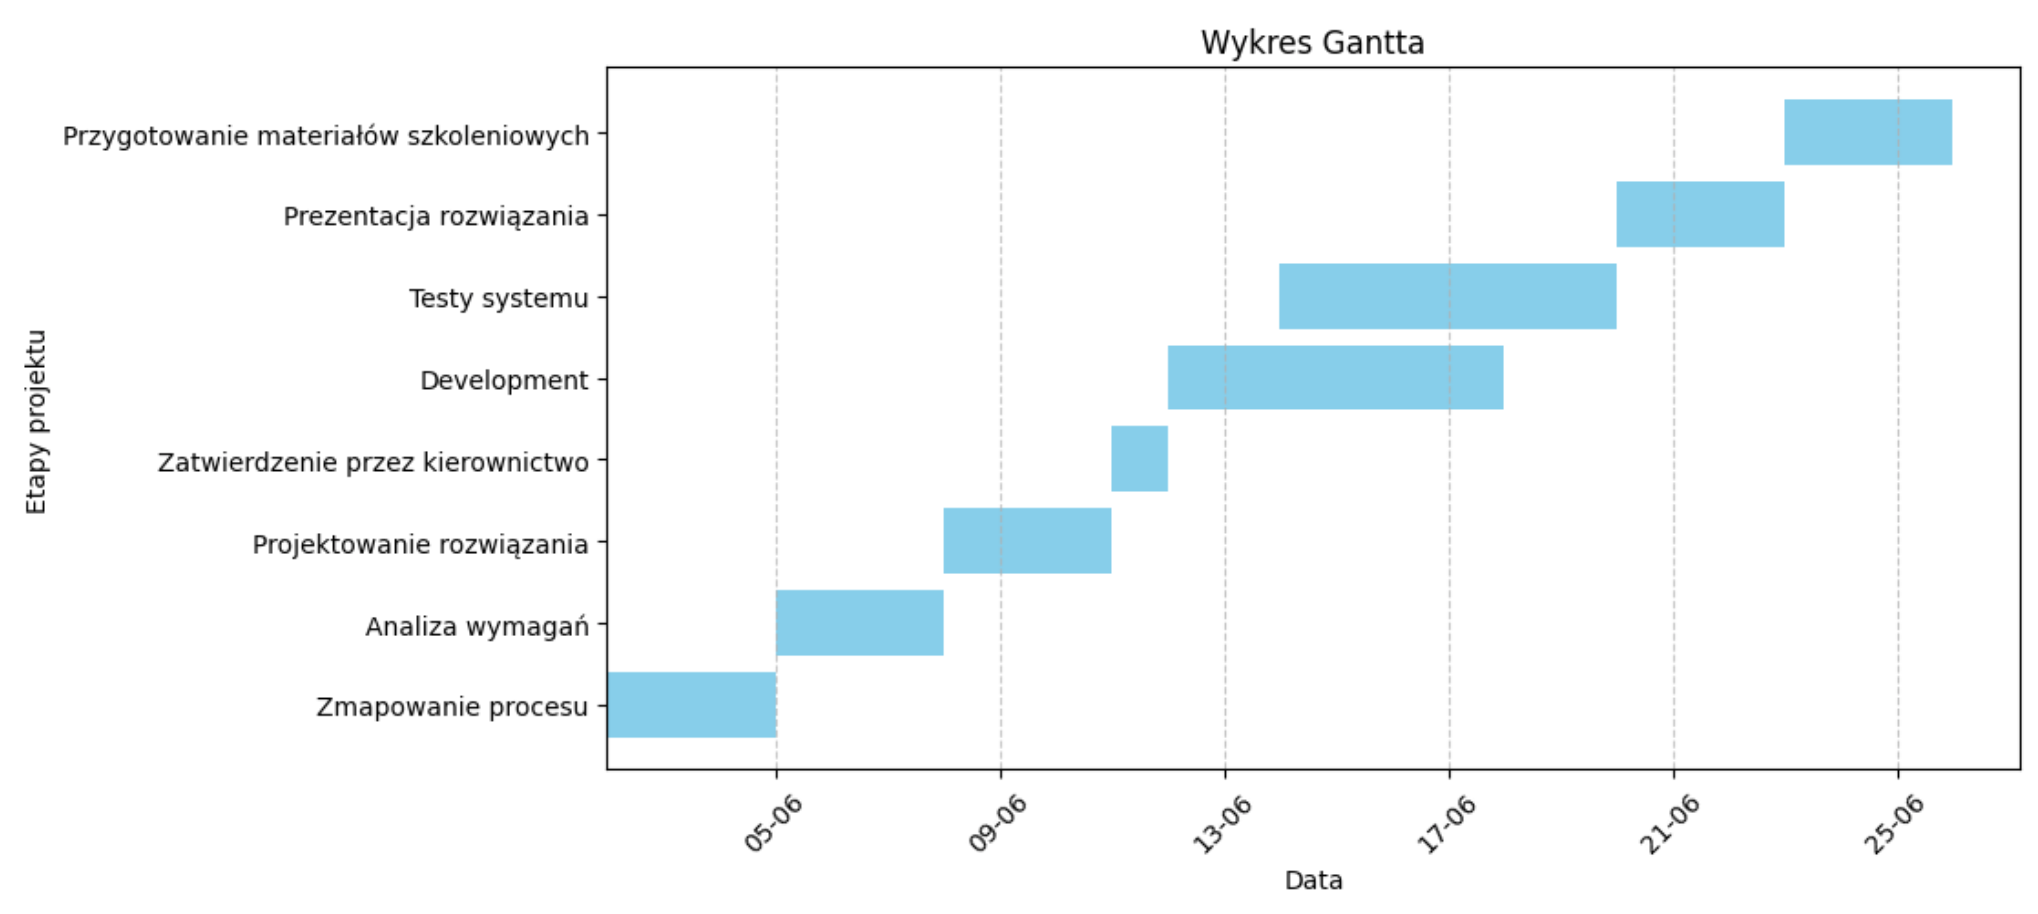
\includegraphics[width=1\linewidth]{rysunki/gantt2.png}
	\caption{Plan pracy przedstawiony na wykresie Gantta, źródło: opracowanie własne}
	\label{rys:registration}
\end{figure}

Pierwszym etapem było zmapowanie istniejącego procesu zarządzania danymi, co pozwoliło na identyfikację obszarów wymagających optymalizacji. Następnie przeprowadzono szczegółową analizę wymagań, uwzględniając potrzeby zarówno organizacyjne, jak i technologiczne. Po zatwierdzeniu specyfikacji przez kierownika projektu nastąpił etap opracowania rozwiązania i konsultacji z kierownictwem inkubatora w celu finalnej akceptacji przyjętej koncepcji.

Proces developmentu obejmował konfigurację środowiska dostępnego dla organizacji, nadanie uprawnień dla odpowiednich grup użytkowników, a także implementację przepływów pracy w \gls{powerautomate} i \gls{powerquery}. Kolejnym krokiem było przeprowadzenie testów systemu, początkowo przez programistę, a następnie przez kierownika projektu, co pozwoliło na weryfikację zgodności funkcjonalnej. Po pozytywnym zakończeniu testów rozwiązanie zostało zaprezentowane przed całym zespołem inkubatora. Ostateczna faza obejmowała opracowanie materiałów szkoleniowych w formie filmu instruktażowego oraz szczegółowego przewodnika krok po kroku, które miały zapewnić płynne wdrożenie systemu w codziennej pracy organizacji.

Harmonogram prac przewidywał realizację całego projektu w ciągu jednego miesiąca. Takie podejście pozwoliło na szybkie wdrożenie optymalizacji, minimalizując zakłócenia w bieżącej działalności inkubatora.
